\ProvidesFile{rutitlepage.dtx}[2022/02/21 v3.0 Radboud University Titlepage]
\documentclass{ltxdoc}
\usepackage{a4wide}
\usepackage{background}
\usepackage{float}
\usepackage{graphicx}
\usepackage{array}
\usepackage[utf8]{inputenc}
\usepackage{rutitlepage}
\usepackage{fancyhdr}
\usepackage[style=ieee]{biblatex}
\usepackage{cryptocode}
\addbibresource{cryptobib/crypto.bib}
\GetFileInfo{rutitlepage.dtx}

\pagestyle{fancy}
\fancyhf{}
\lhead{Bacholer Thesis}
\rhead{Page \thepage}

\backgroundsetup{
   scale=1,
   angle=0,
   opacity=1,
   color=black,
    contents={\begin{tikzpicture}[remember picture, overlay]
      \node at ([yshift=5.9 cm]current page.south)
            {
\includegraphics[width = \paperwidth]{template images/ruhuisstijl2017-en-169-redslide.pdf}} ;
     \end{tikzpicture}}
 }

\title{research proposal}
\author{stijnvandenput }
\date{20 May 2022}

\begin{document}
\maketitleru[
    layout=traditional,
    authors={Stijn Vandenput},
    authorstext={Author:},
    nextpagenr={-1},
    date={20/05/2022},
    institution={Radboud Honours Academy},
    others={Supervisor:}{Martijn Stam\\Bart Mennink},
    course={Bachelor Thesis},
    title={TBD}]

\section*{Abstract}
test \cite{EC:NamRogShr14}
\pagenumbering{roman}
\newpage
\tableofcontents

\newpage
\pagenumbering{arabic}

\section{Introduction}
should consist of:
\begin{itemize}
	\item explaining the challenge
	\item my contribution
\end{itemize}

\section{Preliminaries}
should consist of:
\begin{itemize}
	\item recapping known definitions
	\item primitive definitions
\end{itemize}

\section{Existing AE/DEM notations in more detail}
should consist of:
\begin{itemize}
	\item the def of the two paper, if possible already brought more toward one notation standard
\end{itemize}
\subsection{Existing notation from pkc}
\subsubsection{used primitives}
\begin{itemize}
    \item ADEM: input fixed length tag, fixed length key and variable length message lead to a variable length cythertext. It should be improbable distinguish the cythertexts of two messages. (adversary may choose two cythertexts and has to guess which one of the two is encrypted). The ADEM gives us access to a enc and a dec call.
    
    \item AMAC: input fixed length tag, fixed length key and variable length message lead to a fixed length cythertext. It should be improbable to make a forgery (a pair (key, tag, message, cythertext) that verifies without begin generated by calling O.mac(key, tag, message) first). The AMAC gives us access to a mac and a ver call.
\end{itemize}

\subsubsection{goal}
Each user is provided with two keys, a message and a tag that is bound to the user and does not repeat between users. The message is encrypted using the tag and two keys to generate a cythertext consisting of two parts. First part is Cdem which is the message encrypted with the nonce and the first key while the second part is Cmac that is the mac computed over Cdem, the tag and the second key. Given only one queries to Oenc per user and multiple queries to Odec which always occurs after the Oenc queries, the message should be protected against active adversaries as long as DEM and MAC are secure.

\subsubsection{Sec model}
the security is purely based on the games for the AMAC and ADEM that are visible below where the ADAM calls are replaced with the ADEM' calls. All variables are elaborated in the paper
\begin{figure}[H]
    \centering
    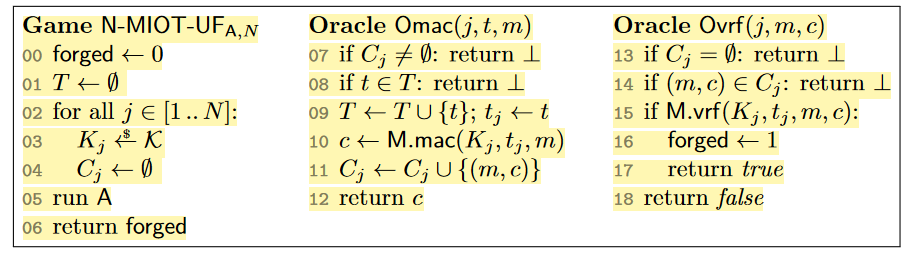
\includegraphics[scale = 0.5]{images/game mac.png}
	\caption{AMAC game}
\end{figure}

\begin{figure}[H]
    \centering
    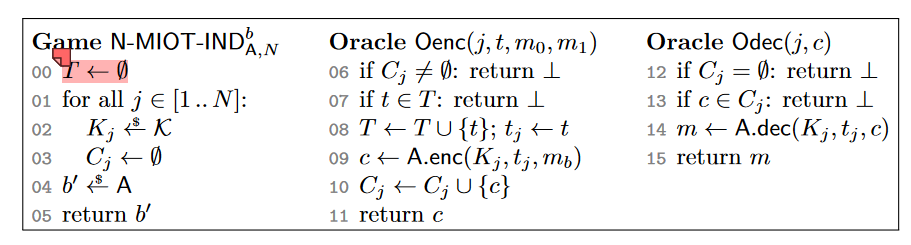
\includegraphics[scale = 0.5]{images/game adem.png}
	\caption{ADEM game}
\end{figure}
with
\begin{figure}[H]
    \centering
    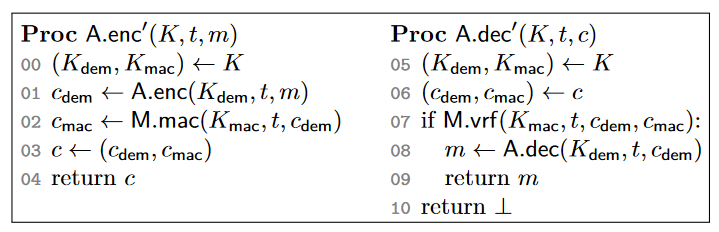
\includegraphics[scale = 0.5]{images/adem amac.png}
	\caption{ADEM' calls}
\end{figure}

\subsection{Existing notation from generic composition reconsidered}
\subsubsection{used primitives}
\subsubsection{goal}
\subsubsection{Sec model}

\section{New Definition}
should consist of:
\begin{itemize}
	\item syntax of the primitive (input,output,correctness,tidiness, expected bounds)
	\item game based code
	\item explanation of the choices made
	\item formal comparison with other choices
\end{itemize}

for now we only look at the nonce based options as the pkc paper does that too.
\subsection{used primitives}
\begin{itemize}
    \item DEM: input fixed length nonce, fixed length key and variable length message lead to a variable length cythertext which should be improbable to distinguish from a random function \$ (adversary has to guess if he is talking to \$ or DEM). The dem gives us access to a enc and dec call.
    
    \item MAC: input fixed length nonce, fix length key and variable length message lead to a fixed length tag that should be improbable to distinguishable from a random function \$ (adversary has to guess if he is talking to \$ or MAC). The MAC gives us access to a mac call.
\end{itemize}

\subsection{goal}
Each user is provided with two keys, a message and a lock that does not repeat between users. The message is encrypted using the lock and two keys. Given only one queries to Oenc per user and multiple queries to Odec which always occurs after the Oenc queries, the message should be protected against active adversaries as long as DEM and MAC are secure.

\subsection{Sec model}
We define the following sec games for the MAC, the DEM and the AE (names will be improved later):

\begin{figure}[H]
    \begin{pchstack}[boxed,center,space=0.5cm]
        \pseudocode[lnstart=-1,linenumbering,head={\textbf{Game} MAC$^M_{A,N}$ }]{
        L \leftarrow \emptyset\\
        \pcfor j \in [1..N]:\\
        \t K_j \leftarrow^\$ K\\
        b' \leftarrow A\\
        \pcreturn b'
        }
        \pseudocode[lnstart=4,linenumbering,head={\textbf{Oracle} Omac(j,l,m)}]{
            \pcif T_j \neq \emptyset: \pcreturn \bot\\
            \pcif l \in L: \pcreturn \bot\\
            L \leftarrow L \cup \{l\}\\
            l_j = l\\
            t \leftarrow M.mac(K_j,l_j,m)\\
            \pcreturn t
        }
    \end{pchstack}
\caption{MAC game where M is either the MAC or a random function \$, adversary A has access to Omac}
\end{figure}

\begin{figure}[H]
    \begin{pchstack}[boxed,center,space=0.5cm]
        \pseudocode[lnstart=-1,linenumbering,head={\textbf{Game} DEM$^E_{A,N}$ }]{
        L \leftarrow \emptyset\\
        \pcfor j \in [1..N]:\\
        \t K_j \leftarrow^\$ K\\
        b' \leftarrow A\\
        \pcreturn b'
        }
        \pseudocode[lnstart=4,linenumbering,head={\textbf{Oracle} Omac(j,l,m)}]{
            \pcif T_j \neq \emptyset: \pcreturn \bot\\
            \pcif l \in L: \pcreturn \bot\\
            L \leftarrow L \cup \{l\}\\
            l_j = l\\
            c \leftarrow E.enc(K_j,l_j,m)\\
            \pcreturn c
        }
    \end{pchstack}
\caption{DEM game where E is either the DEM or a random function \$, adversary A has access to Oenc}
\end{figure}

\begin{figure}[H]
    \begin{pchstack}[boxed,center,space=0.5cm]
        \pseudocode[lnstart=-1,linenumbering,head={\textbf{Game} AE$^{AE}_{A,N}$ }]{
        L \leftarrow \emptyset\\
        \pcfor j \in [1..N]:\\
        \t K_j \leftarrow^\$ K\\
        \t C_j \leftarrow \emptyset\\
        b' \leftarrow A\\
        \pcreturn b'
        }
        \pseudocode[lnstart=5,linenumbering,head={\textbf{Oracle} Oenc(j,l,m)}]{
            \pcif T_j \neq \emptyset: \pcreturn \bot\\
            \pcif l \in L: \pcreturn \bot\\
            L \leftarrow L \cup \{l\}\\
            l_j = l\\
            c \leftarrow AE.enc(K_j,l_j,m)\\
            C_j \leftarrow C_j \cup c\\
            \pcreturn t
        }
        \pseudocode[lnstart=12,linenumbering,head={\textbf{Oracle} Odec(j,m)}]{
            \pcif c_j \neq \emptyset: \pcreturn \bot\\
            \pcif c \in C_j: \pcreturn \bot\\
            m \leftarrow AE.dec(K_j,L_j,c)\\
            \pcreturn m
        }
    \end{pchstack}
\caption{AE game, where AE is either the AE scheme build from the MAC and DEM or a random function \$, adversary A has access to Oenc and Odec}
\end{figure}
\noindent We should consider what the \$ calls should do, there are several cases to consider:
\begin{itemize}
    \item \$ replacing M: \$.mac(k,l,m) calls t = M.mac(k,l,m) then outputs $\bot$ if t is $\bot$ or $\mid t \mid$ random bits otherwise.
    \item \$ replacing E: \$.enc(k,l,m) calls c = E.enc(k,l,m) then outputs $\bot$ if c is $\bot$ or $\mid c \mid$ random bits otherwise.
    \item \$ replacing AE: \$.enc(k,l,m) calls c = AE.enc(k,l,m) then outputs $\bot$ if c is $\bot$ or $\mid c \mid$ random bits otherwise. \$.dec(k,l,c) always returns $\bot$.
\end{itemize}

\section{Constructions}
should consist of:
\begin{itemize}
	\item how to construct the new primitive from old primitives
	\item security bounds + proof
	\item comparison with existing alternatives
\end{itemize}

\noindent The AE schemes should be constructed from the DEM and the MAC. Following General Composition reconsidered, three ways to construct this AE are of interest, namely the ones following from the N1, N2 and N3 scheme. One thing to keep in mind with this that these schemes would originally use associated data. For now we can discard this but it is not proven that the same security results would also follow from this case without associated data. Down here the initial schemes can be found, followed by the AE.enc and AE.dec calls that can we construct following these schemes.
\begin{figure}[H]
    \centering
    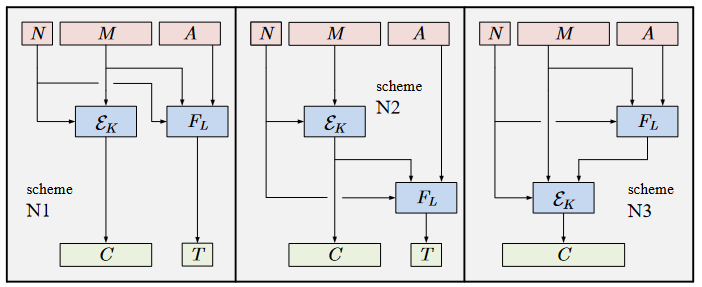
\includegraphics[scale = 0.7]{images/N games.png}
\caption{Original N schemes from Generic Composition reconsidered}
\end{figure}

\begin{figure}[H]
    \begin{pchstack}[boxed,center,space=0.5cm]
        \pseudocode[lnstart=-1,linenumbering,head={AE.enc(k,l,m)}]{
            (k1,k2) \leftarrow k \\
            c' = E.enc(k1,l,m) \\
            t = M.mac(k2,l,m) \\
            c = (c',t)\\
            \pcreturn c
        }
        \pseudocode[lnstart=4,linenumbering,head={AE.dec(k,l,c)}]{
            (k1,k2) \leftarrow k \\
            (c',t) \leftarrow c \\
            m = E.dec(k1,l,c') \\
            t' = M.mac(k2,l,m) \\
            \pcif t = t' : \pcreturn m \\
            \pcelse : \pcreturn \bot
        }
    \end{pchstack}
\caption{Calls based on N1}
\end{figure}

\begin{figure}[H]
    \begin{pchstack}[boxed,center,space=0.5cm]
        \pseudocode[lnstart=-1,linenumbering,head={AE.enc(k,l,m)}]{
            (k1,k2) \leftarrow k\\
            c' = E.enc(k1,l,m)\\
            t = M.mac(k2,l,c')\\
            c = (c',t)\\
            \pcreturn c
        }
        \pseudocode[lnstart=4,linenumbering,head={AE.dec(k,l,c)}]{
            (k1,k2) \leftarrow k\\
            (c',t) \leftarrow c\\
            m = E.dec(k1,l,c')\\
            t' = M.mac(k2,l,c')\\
            \pcif t = t' : \pcreturn m \\
            \pcelse : \pcreturn \bot
        }
    \end{pchstack}
\caption{Calls based on N2}
\end{figure}

\begin{figure}[H]
    \begin{pchstack}[boxed,center,space=0.5cm]
        \pseudocode[lnstart=-1,linenumbering,head={AE.enc(k,l,m)}]{
            (k1,k2) \leftarrow k\\
            t = M.mac(k2,l,m)\\
            m' = m || t\\
            c = E.enc(k1,l,m')\\
            \pcreturn c
        }
        \pseudocode[lnstart=4,linenumbering,head={AE.dec(k,l,c)}]{
            (k1,k2) \leftarrow k\\
            m' = E.dec(k1,l,c)\\
            (m,t) \leftarrow m'\\
            t' = M.mac(k2,l,m)\\
            \pcif t = t' : \pcreturn m \\
            \pcelse : \pcreturn \bot
        }
    \end{pchstack}
\caption{Calls based on N3}
\end{figure}

\section{Use cases}
should consist of:
\begin{itemize}
	\item possible use cases
\end{itemize}

\section{Related Work}
\textbf{Location not final yet}

\section{Conclusion}

\newpage
\printbibliography[heading=bibintoc,title={References}]
\section{Appendix}

\end{document}

\NeedsTeXFormat{LaTeX2e}
\ProvidesPackage{rutitlepage}[2022/02/21 Mart Lubbers]
\RequirePackage{geometry,graphicx,ifpdf,keyval,iflang}
\def\@rutitleauthors{\@author}
\def\@rutitleauthorstext{Aut\IfLanguageName{dutch}{eu}{ho}r:}
\def\@rutitledate{\@date}
\def\@rutitleinst{Radboud Universit\IfLanguageName{dutch}{eit}{y} Nijmegen}
\def\@rutitletitle{\@title}
\def\@rutitlelayout{twentytwo}
\newif\if@rutitlecolour\@rutitlecolourfalse
\define@key{maketitleru}{authors}{\def\@rutitleauthors{#1}}
\define@key{maketitleru}{authorstext}{\def\@rutitleauthorstext{#1}}
\define@key{maketitleru}{colour}[true]{\@rutitlecolourtrue}
\define@key{maketitleru}{course}{\def\@rutitlecourse{#1}}
\define@key{maketitleru}{date}{\def\@rutitledate{#1}}
\define@key{maketitleru}{institution}{\def\@rutitleinst{#1}}
\define@key{maketitleru}{layout}{\def\@rutitlelayout{#1}}
\define@key{maketitleru}{nextpagenr}{\def\@rutitlenextpagenr{#1}}
\define@key{maketitleru}{others}{\def\@rutitleothers{#1}}
\define@key{maketitleru}{subtitle}{\def\@rutitlesubtitle{#1}}
\define@key{maketitleru}{title}{\def\@rutitletitle{#1}}
\newcommand*{\rutitlepage@printothers}[2]{\textit{#1}\\#2}
\newcommand*{\rutitlepage@sepothers}{\\[\baselineskip]}
\newcommand*{\rutitlepage@others}[2]{%
	\rutitlepage@printothers{#1}{#2}%
	\kernel@ifnextchar,{\rutitlepage@sepothers\rutitlepage@otherslist@}\relax}
\newcommand*{\rutitlepage@otherslist}[1]{%
	\expandafter\rutitlepage@others#1}
\def\rutitlepage@otherslist@,#1{\rutitlepage@otherslist{{#1}}}
\newcommand{\rutitle@layout@twentytwo}[0]{
	\newgeometry{left=25mm,top=25mm,right=15mm,bottom=10mm,hmarginratio=1:1}
	\begin{titlepage}%
		\null\vfill%
		\parindent0pt
		\ifdefined\@rutitlecourse\textsc{\LARGE\@rutitlecourse}\\[1.5cm]\fi
		{\Huge\bfseries\@rutitletitle}%
		\ifdefined\@rutitlesubtitle{\\[2\baselineskip]\large\itshape\@rutitlesubtitle\/}\fi\\[4\baselineskip]
		{\Large\scshape\@rutitleauthors}\\[\baselineskip]
		{\large\@rutitledate}
		\vfill

		\ifdefined\@rutitleothers\rutitlepage@otherslist\@rutitleothers\fi
		\vfill

		\hfill
		\ifpdf\includegraphics[width=80mm]{rutitlepage-logo-\IfLanguageName{dutch}{nl-}{}\if@rutitlecolour cmyk\else bw\fi.pdf}\\
		\else\includegraphics[width=80mm]{rutitlepage-logo-\IfLanguageName{dutch}{nl-}{}\if@rutitlecolour cmyk\else bw\fi.eps}\\
		\fi
	\end{titlepage}
	\restoregeometry%
}
\newcommand{\rutitle@layout@seventeen}[0]{
	\newgeometry{left=25mm,top=25mm,right=15mm,bottom=10mm,hmarginratio=1:1}
	\begin{titlepage}%
		\null\vfill%
		\parindent0pt
		{\Huge\bfseries\@rutitletitle}%
		\ifdefined\@rutitlesubtitle{\\[2\baselineskip]\large\itshape\@rutitlesubtitle\/}\fi\\[4\baselineskip]
		{\Large\scshape\@rutitleauthors}\\[\baselineskip]
		{\large\@rutitledate}
		\vfill

		\ifdefined\@rutitleothers\rutitlepage@otherslist\@rutitleothers\fi
		\vfill

		\hfill
		\ifpdf\includegraphics[width=80mm]{rutitlepage-logo-\IfLanguageName{dutch}{nl-}{}\if@rutitlecolour cmyk\else bw\fi.pdf}\\
		\else\includegraphics[width=80mm]{rutitlepage-logo-\IfLanguageName{dutch}{nl-}{}\if@rutitlecolour cmyk\else bw\fi.eps}\\
		\fi
	\end{titlepage}
	\restoregeometry%
}
\newcommand{\rutitle@layout@traditional}[0]{
	\newgeometry{hmarginratio=1:1}
	\begin{titlepage}
		\begin{center}
			\ifdefined\@rutitlecourse\textsc{\LARGE\@rutitlecourse}\\[1.5cm]\fi
			\ifpdf\includegraphics[height=150pt]{rutitlepage-logo.pdf}\\
			\else\includegraphics[height=150pt]{rutitlepage-logo.eps}\\
			\fi
			\vspace{0.4cm}
			\textsc{\Large\@rutitleinst}\\[1cm]
			\hrule
			\vspace{0.4cm}
			\textbf{\large\@rutitletitle}\\[0.4cm]
			\hrule
			\ifdefined\@rutitlesubtitle
				\vspace{0.4cm}
				\textit{\@rutitlesubtitle}\\[1cm]
			\else
				\vspace{2cm}
			\fi
			\begin{minipage}[t]{0.45\textwidth}
				\begin{flushleft}\large
					\textit{\@rutitleauthorstext}\\
					\@rutitleauthors{}
				\end{flushleft}
			\end{minipage}
			\begin{minipage}[t]{0.45\textwidth}
				\begin{flushright}\large
					\ifdefined\@rutitleothers
					\renewcommand{\rutitlepage@printothers}[2]{\textit{##1}\\##2}
					\renewcommand{\rutitlepage@sepothers}[0]{

						\vspace{8mm}}
					\rutitlepage@otherslist\@rutitleothers
					\fi
				\end{flushright}
			\end{minipage}
			\vfill
			{\large\@rutitledate}
		\end{center}
	\end{titlepage}
	\restoregeometry%
}
\newcommand{\maketitleru}[1][]{
	\setkeys{maketitleru}{#1}
	\ifcsname%
		rutitle@layout@\@rutitlelayout\endcsname
		\expandafter\csname rutitle@layout@\@rutitlelayout\endcsname
	\else
		\PackageError{rutitlepage}
			{Unknown layout `\@rutitlelayout'.}
			{The `layout' key of \maketitleru\space contained an unknown layout.\MessageBreak{}
			 Check the package documentation for the possible layouts.}
	\fi
	\ifdefined\@rutitlenextpagenr\setcounter{page}{\@rutitlenextpagenr}\fi%
}